\documentclass{article}
\setcounter{secnumdepth}{0}
%[a4paper, 11pt]
\usepackage{comment} % enables the use of multi-line comments (\ifx \fi) 
\usepackage{fullpage} % changes the margin

\usepackage{graphicx}
%\usepackage{lscape}
%\usepackage{rotating}
\usepackage{pdflscape}
\usepackage{wrapfig}
\usepackage{gensymb}
\usepackage{graphicx}

\renewcommand{\labelenumii}{\theenumii}
\renewcommand{\theenumii}{\theenumi.\arabic{enumii}.}

\usepackage{enumitem}
\usepackage{subcaption}
%\usepackage[]{algorithm2e}
%\usepackage{pgffor}
\usepackage[T1]{fontenc}
\usepackage{xcolor}

\newcommand{\CMwidth}{-1.7cm}
\newcommand{\CMheight}{2.7cm}

\usepackage{hyperref}

\setcounter{secnumdepth}{5}% Include \subsubsection in ToC

\def\changemargin#1#2{\list{}{\rightmargin#2\leftmargin#1}\item[]}
\let\endchangemargin=\endlist 

\begin{document}
%Header-Make sure you update this information!!!!
%\noindent
%\large\textbf{Post/Pre-Lab X Report} \hfill \textbf{FirstName LastName} \\
%\normalsize ECE 100-003 \hfill Teammates: Student1, Student2 \\
%Prof. Oruklu \hfill Lab Date: XX/XX/XX \\
%TA: Adam Sumner \hfill Due Date: XX/XX/XX

\title{Dissertation: Hybrid Methods for Finite Element Meshing}
\author{Jack Bradbrook (psyjb4)}
\date{April 5, 2017}
\maketitle

\tableofcontents

\newpage

\section{Introduction}

The overall aim of this project is to perform the task of refining a Finite Element Mesh (FEM) using a stress based method as is typical of FEM refinement in conjunction with an approach that uses techniques from Artificial Intelligence and Machine Learning. It should be possible to reason about the quality of a mesh produced using both methods analytically in order to evaluate the success of the approach and potential for continued use.\\

\noindent
Finite Element Analysis (FEA) is a method widely used across different engineering domains to simulate structures under certain conditions. The method works by taking a geometry defined in continuous terms, discretize it into a mesh system before calculating the property values for each of the discrete elements. This allows engineers to observe the effect the conditions have on the entire structure, see figure 1. \\ 

\noindent
Success of the project will be determined by implementation of a system that is able to combine the two approaches described above in order to refine a mesh to of a quality comparable to that of a successful stress based method.


\section{Motivation and Background}

Over the past forty years FEA has emerged as a prominent technology for simulating complex real world engineering problems \cite{cite0, DolsakPaper94}. FEA works by solving a system of differential equations with each equation representing a single element in a geometric mesh. By doing this FEA is able to generate highly accurate approximations for the properties of complex physical systems \cite{DolsakPaper94} \cite{IntroductionToFE}. The method can also be highly computationally expensive with the complexity typically increasing exponentially with the model size \cite{DolsakPaper94}. Analysis therefore proves to be highly time consuming and costly for individuals and organisations to conduct \cite{ConsultRuleIntelltSystemFE}. \cite{cite03}\\


\subsection{Properties of finite element models}
Although this dissertation is computer science oriented as opposed to mechanical engineering it's still important to briefly describe the general principals and properties that underlie the FE method in order to have a general appreciation for how the design and evaluation of the final software system was conducted. \\ 

\noindent
Finite Element Models have several key properties that need to be specified by the engineers who create them, the configuration of these properties greatly determine the results obtained from the models execution. The first of these properties that an FE model posesses is the mesh. The mesh is constructed out of nodes, points which act as intersections between the second componet- elements which are either a polygon or a polyhedron between the nodes. Nodes and elements are important concepts as they provide the theoretical framework for reasoning about the other properties of a mesh and hence the overall quality of the model \cite{IntroductionToFE}.\\ 

\noindent
In addition to the nodes and elements FE models also contain inputs and constraints. Inputs can be thought of as the phenomena which is acting on the structure and consequently inducing some sort of physical effect on it such as a force. These are used to represent the external conditions the structure will be exposed to when present in an environment. \\

% elements can be different types which have different types, typical types
% triangles and squares. 

\noindent
Constraints are another fundamental concept important when performing FE analysis that describe where the model is attached to the outside world. When computing stresses induced through the model there needs to be an area through which the stresses are assumed to leave. FEA is only able to calculate the path of the stresses through the model and thus the overall stress at given points using the law of conservation of energy i.e. energy cannot be created or destroyed meaning that any energy provided to the system as input through for example force needs a means by which to leave it, the constraint. \\

\noindent
For example in figure 6 showing a suspension bridge model the simulation is to be run with the forces are induced upon the cables and the towers in the negative x direction as represented by the green vectors. The corresponding constraint area through which the force must leave is specified as the base of each bridge pillar and represented by multiple red arrows on each corresponding corner.\\

\noindent
The final piece of information needed in order to calculate the stresses through the model is material data. Material data is associated with the models elements and is usually defined using two main parameters which are:

\begin{itemize}
\item Youngs Modulus
\item Poissons ratio
\end{itemize}

For the sake of simplicity all structures used to evaluate the final software solution have assumed steel as their material property. 

\noindent
which must be made when conducting


\subsection{Limitations and general considerations}
\noindent
An important consideration when conducting FEA is the trade-off of a models accuracy against the time in which it can be solved. A major variable determining this trade-off is the models mesh structure which discretizes the problem so that simulation can be run on it. A mesh that is finer is more computationally expensive but also produces results of greater accuracy. It is therefore desirable to generate a mesh which is fine where accuracy is most needed but coarse where it is not \cite{cite04}. \\

\noindent
In every type of analysis that the FE method is used for (thermal, structural, fluid flow, electrical) there is a specific differential equation associated with each of the elements. In order to achieve overall convergence of the model the equations must be solved simultaneously to achieve a value for each of the discrete elements \cite{IntroductionToFE}. For this dissertation project attention will be given specifically to the problem of FEA meshing in the context of static structural analysis where the value calculated across each element is its stress. It makes sense to work on hybrid mesh refinement in the context of static structural analysis as it is likely the most common engineering application of the method and as such has the largest body of research that is relevant \cite{DolsakPaper94}\cite{IntroductionToFE}.\\

\noindent
For engineers the value obtained through computing the stresses under a particular set of conditions is feedback on the quality of their design. Ideally the results from an analysis will provide a good understanding of where the design is weak and how concentrated this weakness is. This information is used to either help verify the designs' quality or alternatively inform changes to its geometry or material properties so as to reduce stress on subsequent analysis \cite{cite06}.\\

\noindent
To understand the gradient of stress within a part of the model the mesh needs to be designed carefully. As each element can only display values calculated from its edge nodes a smooth gradient requires a higher concentration of elements in areas under higher stress. A high quality mesh is therefore considered to have a higher concentration of elements in areas of predicted high stress while retaining lower concentration elsewhere, thereby revealing weaknesses in the design while minimising the models runtime.\\

\noindent
Traditionally the automated mesh refinement process consists of computing stresses for a model with an initial coarse mesh and low computation cost, once rough stresses have been computed the elements in areas of higher stress can be divided recursively into additional elements in order to achieve smoother gradients on further executions \cite{cite03}. Figure 1 shows a mesh which has been refined in an area of higher stress thus providing a clearer indication of a components weakness. \\ 

\noindent
Unfortunately for many large models this method for refining a mesh is still excessively costly \cite{DolsakPaper91}. It therefore seems worth investigating use of alternative approaches posed by the field of computer science and artificial intelligence that could support the traditional high stress meshing approach. 

\begin{figure}
  \centerline{\includegraphics[width=110mm, scale=0.5]{stressedCorner.png}}
  \caption{Mesh refinement in corner under high stress image source: (\cite{HighStressCorner})}
  \label{fig:boat1}
\end{figure}

\section{Related Work}

Many approaches have so far been taken in an attempt to improve a computer's ability to perform the task of finite element meshing. The following subsections present an overview of the research conducted for the various aspects of the project which are more explicitly outlined under ``Aims and Objectives"

\subsection{Traditional Stress refinement methods}

A number of methods exist to perform mesh refinement based on a stress gradient for a mesh, with the most common being higherarchical refinementent also known as h-refinement and relocation refinement or r-refinement\cite{HandPRefinements} \cite{RRefinement}\\ 

\noindent
\textbf{h-refinement: }
H-refinement is the process of recursively refining a mesh by splitting elements into additional sub elements. This process can be performed for elements with both both triangular and quadrilateral shapes. \cite{HandPRefinements}. \\ 

\noindent
\textbf{r-refinement: }
R-refinement is a method which attempts to improve the quality of the stress gradient without the alteration of the mesh element count and thus the computational cost. This is achieved by the relocation of elements within the mesh which effectively increases the size of elements in areas of low stress, while reducing the size in areas where stress is high \cite{RRefinement}.


\subsection{Uses of Artificial Intelligence and Machine Learning}

\noindent
Within the domains of AI and machine learning methods such as neural networks \cite{NeuralNetworks}, case based reasoning \cite{caseBasedReasoning} and inductive logic programming \cite{DolsakPaper94} have all been adopted to facilitate generation of meshes comparable to that of human experts.  Similarly there has also been effort to combine multiple numerical methods simultaneously for solving re meshing problems \cite{TraditionalHybridRefinement} although effort to combine the two approaches does not appear to have so far been made.\\ 

\noindent
Due to the difficulty of obtaining meshes which hold commercial interest the majority of researchers working in this field have had to result to the use of training sets developed within academia \cite{DolsakPaper91}. The primary issue associated with this is that often the training data does not exhibit the level of complexity that you would expect in many industrial sectors. Many researchers must accept this as a limitation or agree commercial terms with an organisation in order to gain access to their models \cite{DittmerMeshQualityMet}.\\ 

\noindent
Having reviewed a variety of different AI based applications to FE the use of Inductive Logic Programming (ILP) used by Bojan Dolsak et al is of greatest interest. ILP is a machine learning method first presented by Stephen Muggleton in his 1991 paper ``Inductive Logic Programming" \cite{MuggletonILP}. Muggleton suggests that the traditional approaches of machine learning which rely on use of extensive data sets and statistical analysis are poor in the case of many real world problems for which data is not available \cite{ILPYoutubeLecture}. Muggleton cites Human learning as an example of use of ILP style techniques where understanding of new concepts is achieved not through crunching large volumes of data points but instead  the use of induction on a relatively concise set of background facts and examples obtained from previous life experiances \cite{ILPYoutubeLecture}. \\ 

\noindent
ILP uses three types of input information in order to hypothesise additional facts about the system. These three types of input information are: \\ 

\begin{itemize}
\item Positive examples  of what constitutes an area that is well meshed
\item Negative example of areas that are poorly meshed
\item Background facts
\end{itemize}

\noindent
Using this information ILP is capable of hypothesising rules by determining which rules can exist within the system where given the set of background facts all positive examples are satisfied while few or none of the negative examples are. Although ILP requires a body of additional metadata associated with each mesh this is easier to obtain making ILP a highly practical solution. Along with his publication Muggletons also released his implementation of an ILP algorithm as a program titled ``Golem" \cite{Golem}, Golem was applied by Dolsak to the problem of mesh refinement with a training set of just five meshes \cite{DolsakPaper94}. The resulting rule set when applied to subsequent models was able to correctly classify and re mesh areas with an average accuracy of 78\% for a range of geometries \cite{DolsakPaper94} \cite{appOfILPToFEMeshDesign}. \\

\noindent
Dolsak's choice of metadata for the ILP method to generate mesh rules is based on the classification of edges within the FE model which he knew to be crucial to determining their strength. For example if it is know that an edge within the model has a force applied close to it based on the initial model conditions then other edges that intersect it should be meshed to have a greater concerntration of adjacent elements prior to model execution. \cite{DolsakPaper91} \cite{appOfILPToFEMeshDesign}.\\ 

\noindent
The format of the rules make them attractive for experimenting with as part of a hybrid method since the method determines how to refine the mesh based on the arrangement of edges. This detail of analysis of the mesh is at a comparable detail to that of a traditional splitting method such as h-refinement which will likely to improve the ease at which the two methods can be combined simultaneously in the latter stages of the project. \\ 

\subsection{Quality metrics}
\noindent
Finally work has also been done on establishing valid metrics for assessing the quality of a mesh automatically \cite{DittmerMeshQualityMet, NeuralNetworks} Metrics for meshes have been research far more extensively that AI methods due to their use for comparing different stress based refinements. There are also cases of common metrics being used for industrial meshing applications \cite{DittmerMeshQualityMet}. Although there are metrics for assessing a mesh on a global level such as element count score \cite{DittmerMeshQualityMet} the consensus is that due to the variation in meshes this is less reliable than assessing quality based on the properties of individual elements within the mesh \cite{DittmerMeshQualityMet} \\

\begin{figure}
  \centerline{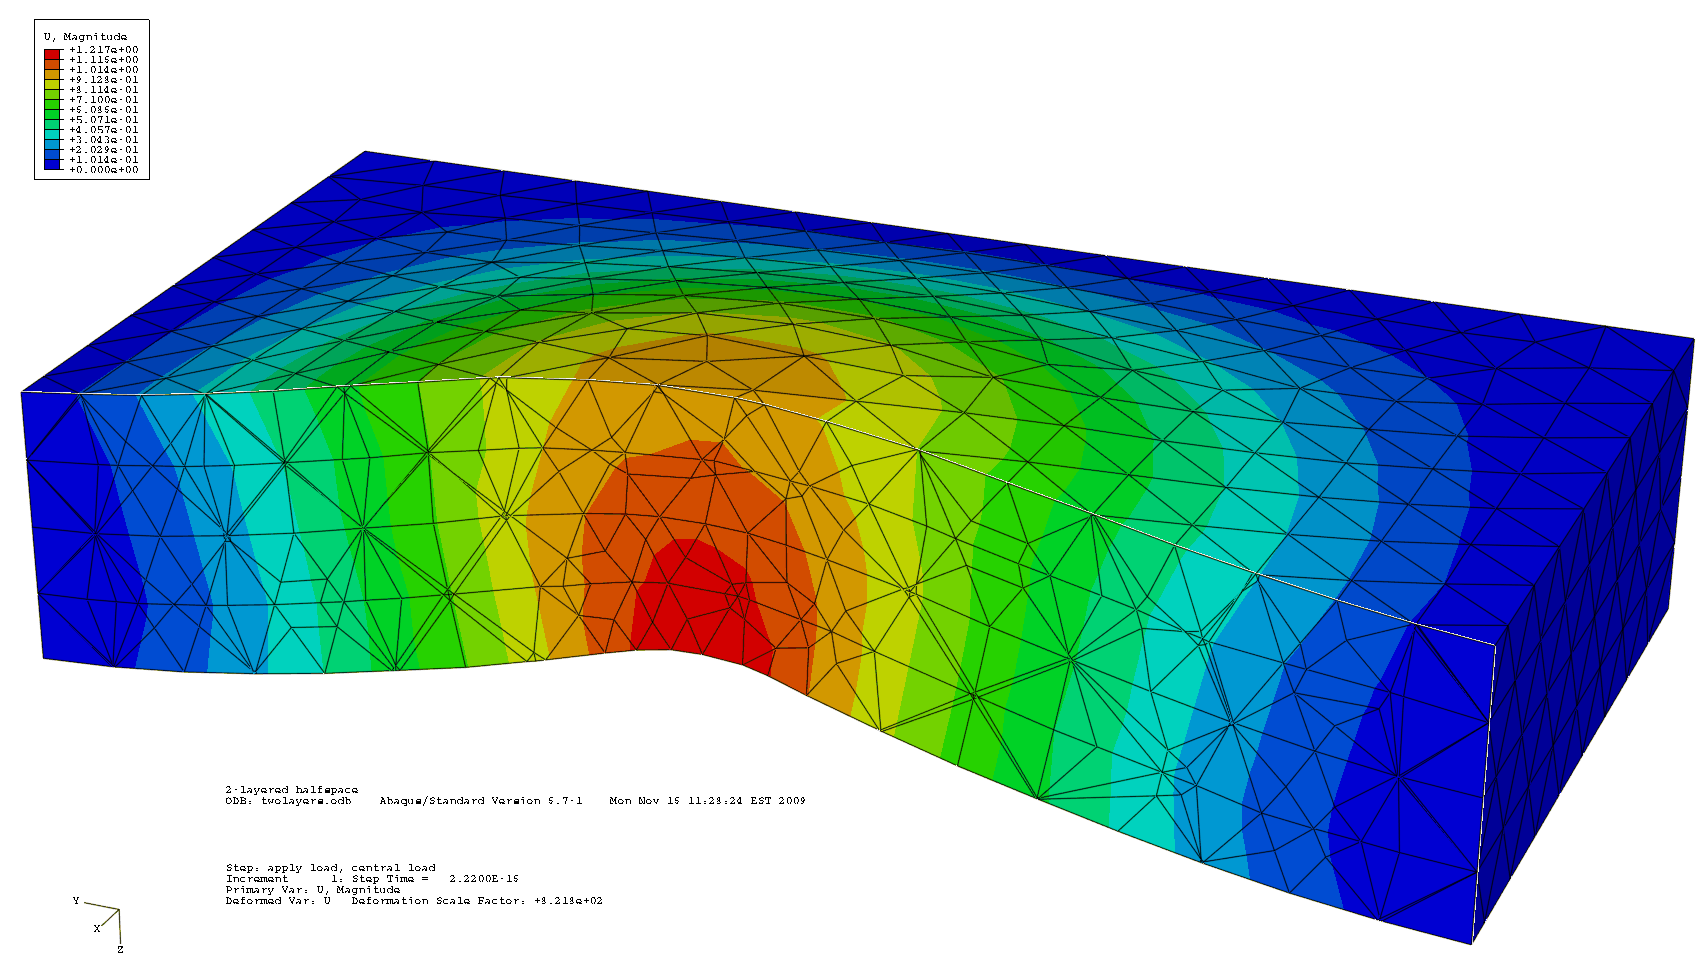
\includegraphics[width=120mm, scale=1]{MeshQualityDeterioration.png}}
  \caption{Example of how elements can be distorted in order to fit a geometry which will result in deterioration of gradient quality (image source: \cite{PoorFEElementShapes})}
\end{figure}


\noindent
Localised metrics associated with the quality of each element have shown to be accurate for predicting the overall quality of a mesh when taking the average for each metric across all elements \cite{DittmerMeshQualityMet}. The quality of an elements shape is important since the stress values which are computed for the area within the element are calculated using the stress values at each of the nodes which enclose it \cite{IntroductionToFE}. Elements are typically deformed near parts of the geometry where its shape simply does not allow a uniform element to be placed, an example of where this has occurred can be seen in figure 2.\\ 

\noindent
Some key shape metrics identified by Dittmer et al include (ideal values are for elements of quadrilateral type as used in  the current prototypes):

\begin{enumerate}[label=\Alph*]
\item Aspect ratio – longest side / shortest side, ideal value is 1
\item Maximum corner angle - widest internal angle to element, ideal is 90\degree
\item Maximum parallel deviation - how skewed the element is, ideal is 0\degree
\end{enumerate}

\section{Description of the work}
\subsection{Aims and Objectives}
The aim of this project was to design, build and analyse a system for refining a mesh by combining a method from the domain of AI or machine learning with a stress based refinement method. The desirable end result will be a hybrid method of meshing which produces reasonably good solution accuracy whilst requiring less user intervention and reduced computational cost.\\

\noindent
The project can be broken into thee main sections of research and implementation which can each be considered a high level objective:\\ 

\begin{enumerate}[label=\Alph*]

\item The first objective is to research and develop both a traditional stress refinement and an AI re meshing algorithm developed by industry or by academia. These algorithms should be able to run independently on a set of example models.

\item Secondly a process will need to be devised for combining the two re meshing methods to varying degrees will be required. This will make it possible to test the effects of a hybrid method across the same set of models. Through this it can be established whether there is notable benefit to combining the different approaches and if so to what degree is it effective.

\item The third objective will be to use justifiable metrics for assessing the quality of a given mesh. This will allow for a much greater range of hybrid variations to be tried without requiring inspection from an expert. 
\end{enumerate}

\section{System specification}
To demonstrate success in achieving the objectives of the project it is important to have tractability from the requirements through to the solution and lastly verification and validation. This section describes the current systems \textit{functional requirements} (what the system will do) and \textit{non-functional} requirements (its constraints) based upon evaluation of the research I have conducted in conjunction with discussions with the project supervisor: Dr Jason Atkin. Functional requirements have primarily been listed under their respective high level subsystems that are responsible for encapsulating their functionality. \\ 

\noindent
Although it has not been developed as part of the project the application responsible for solving the finite element models has been included as part of the systems requirements since it highly influences the overall scope of the project and much of the design associated with other subsystems which were developed for the project. \\ 

\section{Functional Requirements}

\begin{enumerate}
\item FE integration: System will be able to interface with a third party finite element application

\begin{enumerate}
\item The finite element applications solver must be able to solve a mesh based on its model configuration.
\item The finite element applications solver must be able to execute a model programmatically
\item The finite element applications solver must be able to output stress data at different points on the mesh.
\item The finite element application will provide a graphical representation of the model.
\item It will be possible to manipulate the model that the finite element application uses programmatically.
\item It should be possible to manipulate the model that the finite element application uses from within its graphical user interface.
\end{enumerate}

\item Mesh refinement: System will be able to perform different kinds of finite element mesh refinement

\begin{enumerate}
\item The system will be able to refine a finite element mesh using a stress based refinement method
\item The system will be able to refine a finite element mesh using a non-stress based refinement method

\item A non stress based refinement method will adapt the mesh using background information about mesh design which has been previously trained.

\item The system will be able to combine the two methods to produce a coherent mesh which the FE application is able to successfully solve in order to obtain results for stress and displacement.
\item The system will be able to combine both methods to varying degrees will be performed automatically by the system without direct user intervention.
\item The system will re mesh using both stress and non-stress based refinement using quadrilateral elements.
\item System will adapt weighting associated with each method based upon the metrics computer for the mesh in the systems previous iteration.
\end{enumerate}

\item Quality assessment: System will provide the operator with results about the quality of meshes based on metrics obtained from research.

\begin{enumerate}
\item An assessment will be conducted automatically for every mesh iteration that occurs.
\item System will assess quality based on a variety of metrics to ensure overall robustness of measurement. 
\item The metrics will be computed for both individual elements within the model and for the entire mesh.
\end{enumerate}
\end{enumerate}

\section{Non-Functional Requirements}


\textbf{Design:} The system architecture will be developed using the object oriented design principals of SOLID to allow for clear interfaces between the different functional components. Functional programming practices will be adopted through use of the .NET Language Integrated Query or LINQ framework. This will help to simplify the code and improve reliability. Where functions and classes are written their length will be kept to a minimum to reduce complexity and allow for reuse wherever possible. \\ 

\noindent
\textbf{Documentation:} The system will be comprehensively documented at both a code level and at an architecture level. At a code level C\# doc comments will be written to provide a comprehensive summary of each function. This will allow the tool Doxygen \cite{Doxygen} to generate a full set of developer documentation upon completion of the software implementation which will be included as an appendix. Doc comments will also help to encourage small functions. \\

\noindent
\textbf{General applicability:} In order to demonstrate that hybrid methods are a feasible means of approaching meshing problems the resulting software should be able to successfully execute on a range of models with varying geometry. The range of geometries should be representative of typical structural variation.


\section{System Design}


\subsection{System Overview}
Determining the overall design of the system was initially hard since it was not clear exactly how many subsystems would be needed to mesh, evaluate and interface with LISA, what was clear was that the system would essentially be performing an optimisation procedure and as such needed to be driven iteratively towards a goal. 

 It was therefore important to ensure the system maintained a modular architecture with well defined interfaces in order to allow for subsystems to be easily added and modified as the project progressed.


\begin{figure}
  \centerline{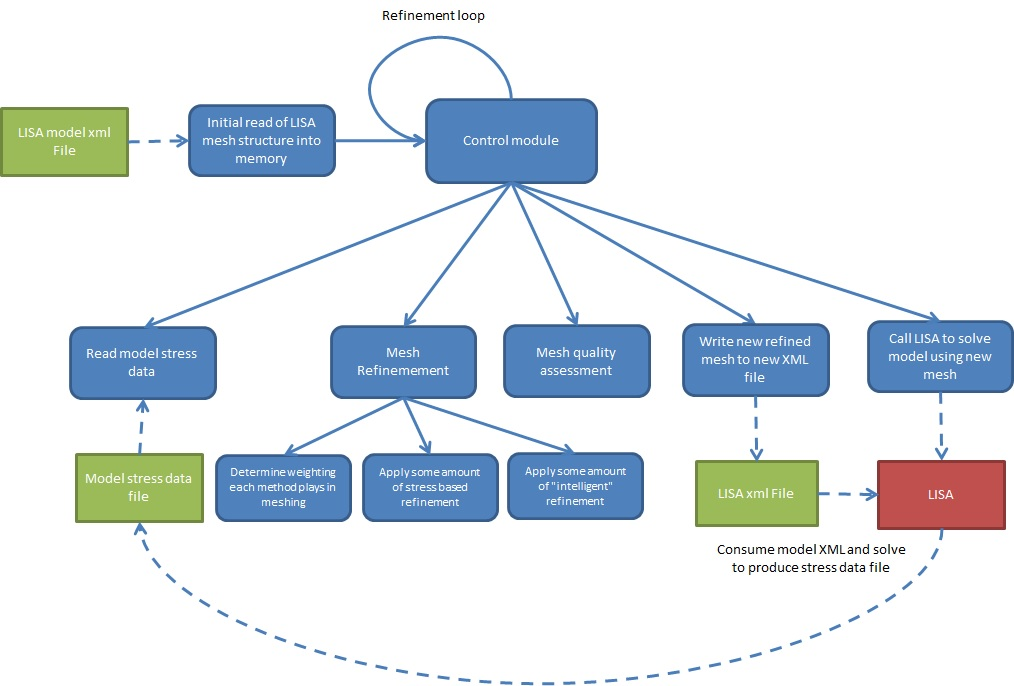
\includegraphics[width=150mm, scale=1]{SystemDesignDiagram.jpeg}}
  \caption{High level design of the system with its different modules}
  \label{fig:h-refinementImp}
\end{figure}


\subsection{Modular Architecture}
The modular architecture allows meshing algorithms and metrics for calculating mesh quality could be swapped interchanged was an important consideration in the design of the system. At best the quality of the output could be predicted for each method before it was integrated into the system and executed in a range of different scenarios. To have tightly coupled these individual components would have rendered the overall system a failure in the event that any one of them performed greatly worse than expected. Instead the loose coupling of the architecture has enabled the system to be considered as more of a framework for testing the effects of combining heuristic knowledge of a Finite element problem with a stress based refinement method.

Although the system was highly modular It was also still desirable to maintain a hierarchy within the classes so that smaller components could be developed independently and contained within the larger ones. Composition was therefore generally favoured over inheritance as a means of building the architecture. 

Static classes and methods were also used when needing to write utility functions that were required by multiple high level subsystems and therefore did no fit especially well into any particular one. Examples of these are generic vector algebra operations such as dot product, matrix determinants and normal vectors.

%\subsection{Mesh improvement Loop}
%As with many optimisation problems the refinement process is driven iteratively through a loop. Within the main loop all %interfacing with LISA, Mesh refinement and analysis is conducted which results in an updated version of the model that can be %handed to the subsequent iteration.


\subsection{Input Files}
The system requires three basic input files which should be placed within a directory that is given to the program as as parameter, these are files are:

\begin{itemize}
\item A structural model represented as a .liml file which LISA can solve
\item A 
\item A JSON file containing important edges as identified by an engineer 
along with associated meta data.
\end{itemize}


\subsection{Multi Threading}
To allow allow for better performance when evaluating a range of different weightings of the stress and heuristic methods multi threading was used to allow each configuration to be run independently of the others. When started each thread creates its own directory which it copies the three input files to and runs for its designating weighting configuration. Use of multi threading made assessment of the system much more rapid in the later stages of the project.



%what happens for each loop iteration


\subsection{Simulation Data Model}
Writing an API for LISA was the first clear stage of development for my project for which a design had to be considered. The API was crucial in order to program the more complex aspects using basic operations and avoid having to regularly perform direct string manipulation of the input files in order to manipulate the model. \\

\noindent
When the first re-meshing iteration occurs the system needs to read the input .liml file into an equivalent class model, diagrams for which can be seen in figure 4 below. Each class in this model contains corresponding data and methods used to represent and manipulate the model. These methods are then used by the different refinement methods that exist in the different optimisation classes to alter the mesh, this adapted version of the mesh represented as a data model can then be assessed by the module responsible for validating mesh quality before finally being written back to a .liml file for LISA to solve on the subsequent iteration. When designing the data model to represent the state within LISA it was desirable to maintain coherence with the structure specified by LISA as closely as possible, this allowed for the data model to more easily be serialised when communicating with LISA without errors resulting from inconsistencies between the two representations. 

\begin{figure}[!h]
\centering
\begin{subfigure}{.5\textwidth}
  \centering
  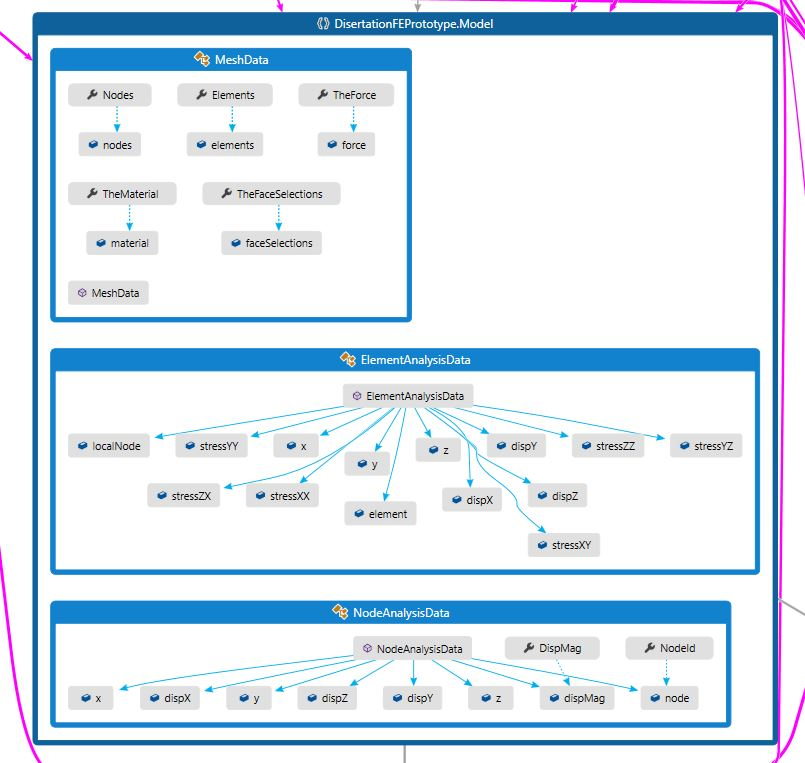
\includegraphics[width=0.9\linewidth]{DissoFEProto-Model.jpg}
  \caption{Model classes}
  \label{fig:sub1}
\end{subfigure}%
\begin{subfigure}{.5\textwidth}
  \centering
  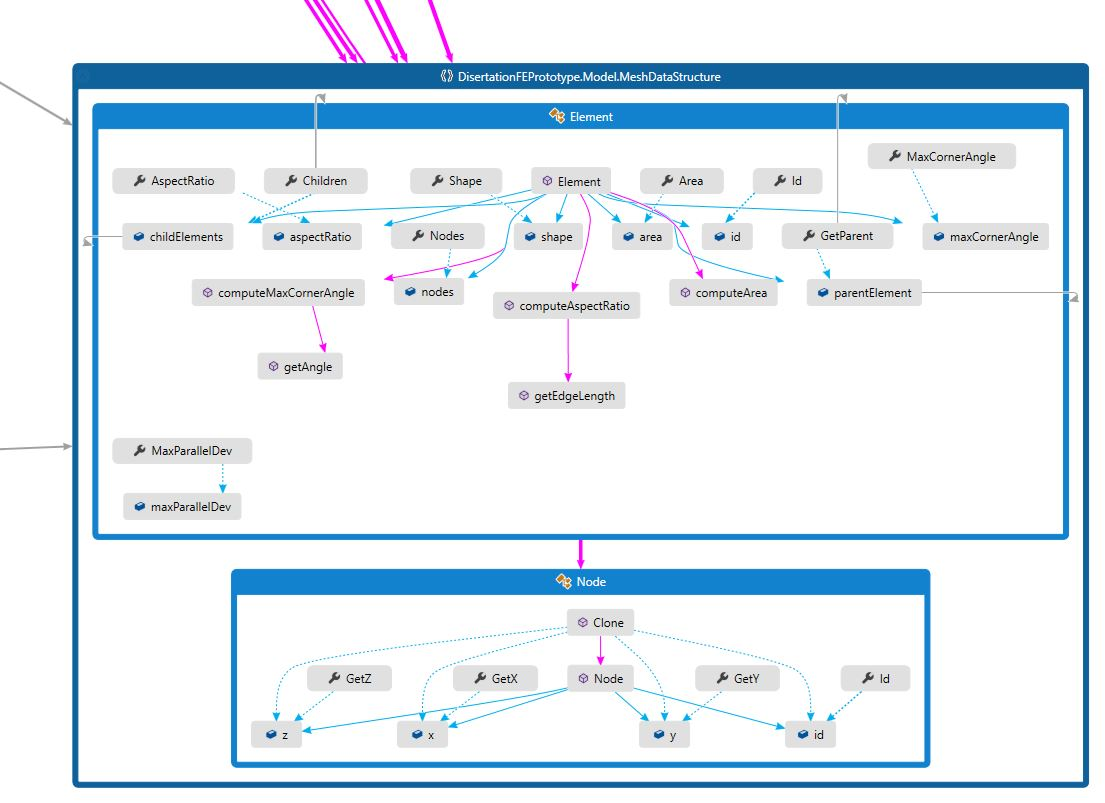
\includegraphics[width=0.9\linewidth]{DissoFEProto-ElemNode.jpg}
  \caption{Element and Node classes}
  \label{fig:sub2}
\end{subfigure}
\label{fig:test}
\end{figure}

\begin{figure}
\centering
\begin{subfigure}{.5\textwidth}
  \centering
  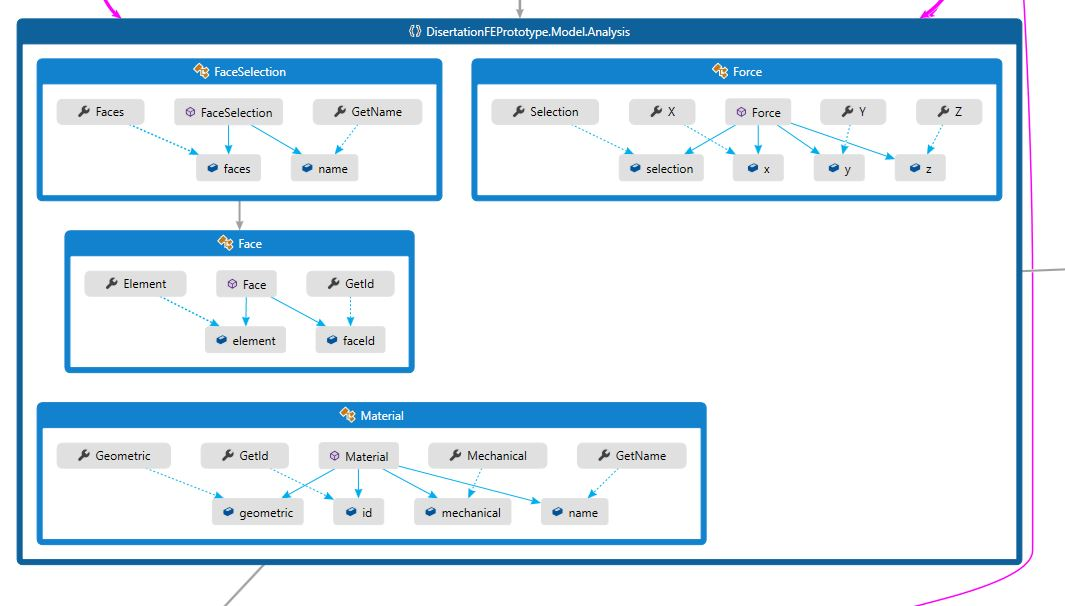
\includegraphics[width=0.9\linewidth]{DissoFEProto-ModelAnalysis.jpg}
  \caption{Model Analysis classes}
  \label{fig:sub1}
\end{subfigure}%
\begin{subfigure}{.5\textwidth}
  \centering
  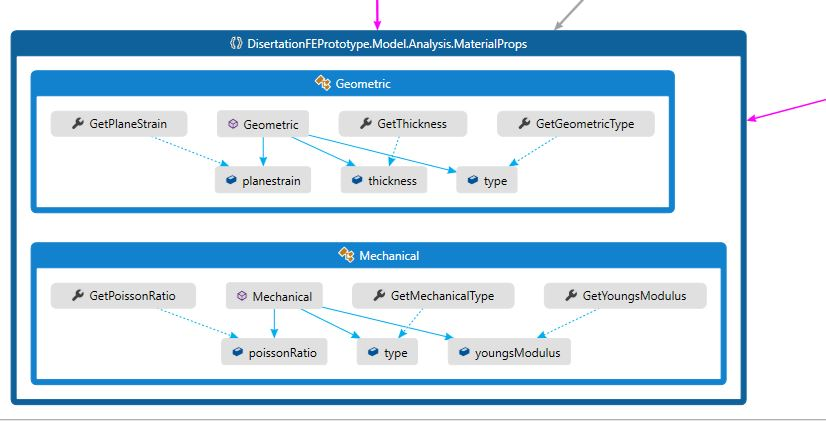
\includegraphics[width=0.9\linewidth]{DissoFEProto-MaterialProps.jpg}
  \caption{Material Property classes}
  \label{fig:sub2}
\end{subfigure}
\label{fig:test}
\caption{Class model to represent .liml file structure used by LISA}
\end{figure}

\clearpage
\noindent
One aspect of the data models design which greatly adds to the systems flexibility is the hierarchical design for representing the various Element types. At the root of this structure is the IElement interface, all new Element types must adhere to this in order for the various refinement methods to run. Implementing the interface are a range of abstract classes such as ``SquareBasedElem" and ``TriangleBasedElem" These classes are designed to contain methods that are generally applicable for calculating metrics and re meshing individual elements for elements of this type that are both in two and three dimensions. This is powerful since computing this for a 3d element is simply a reduction of the method for a 2d element over every face which comprises the 3d one. Finally underneath this level are the concrete classes which represent each specific type of element with its own bespoke characteristics. \\ 

\begin{figure}
  \centerline{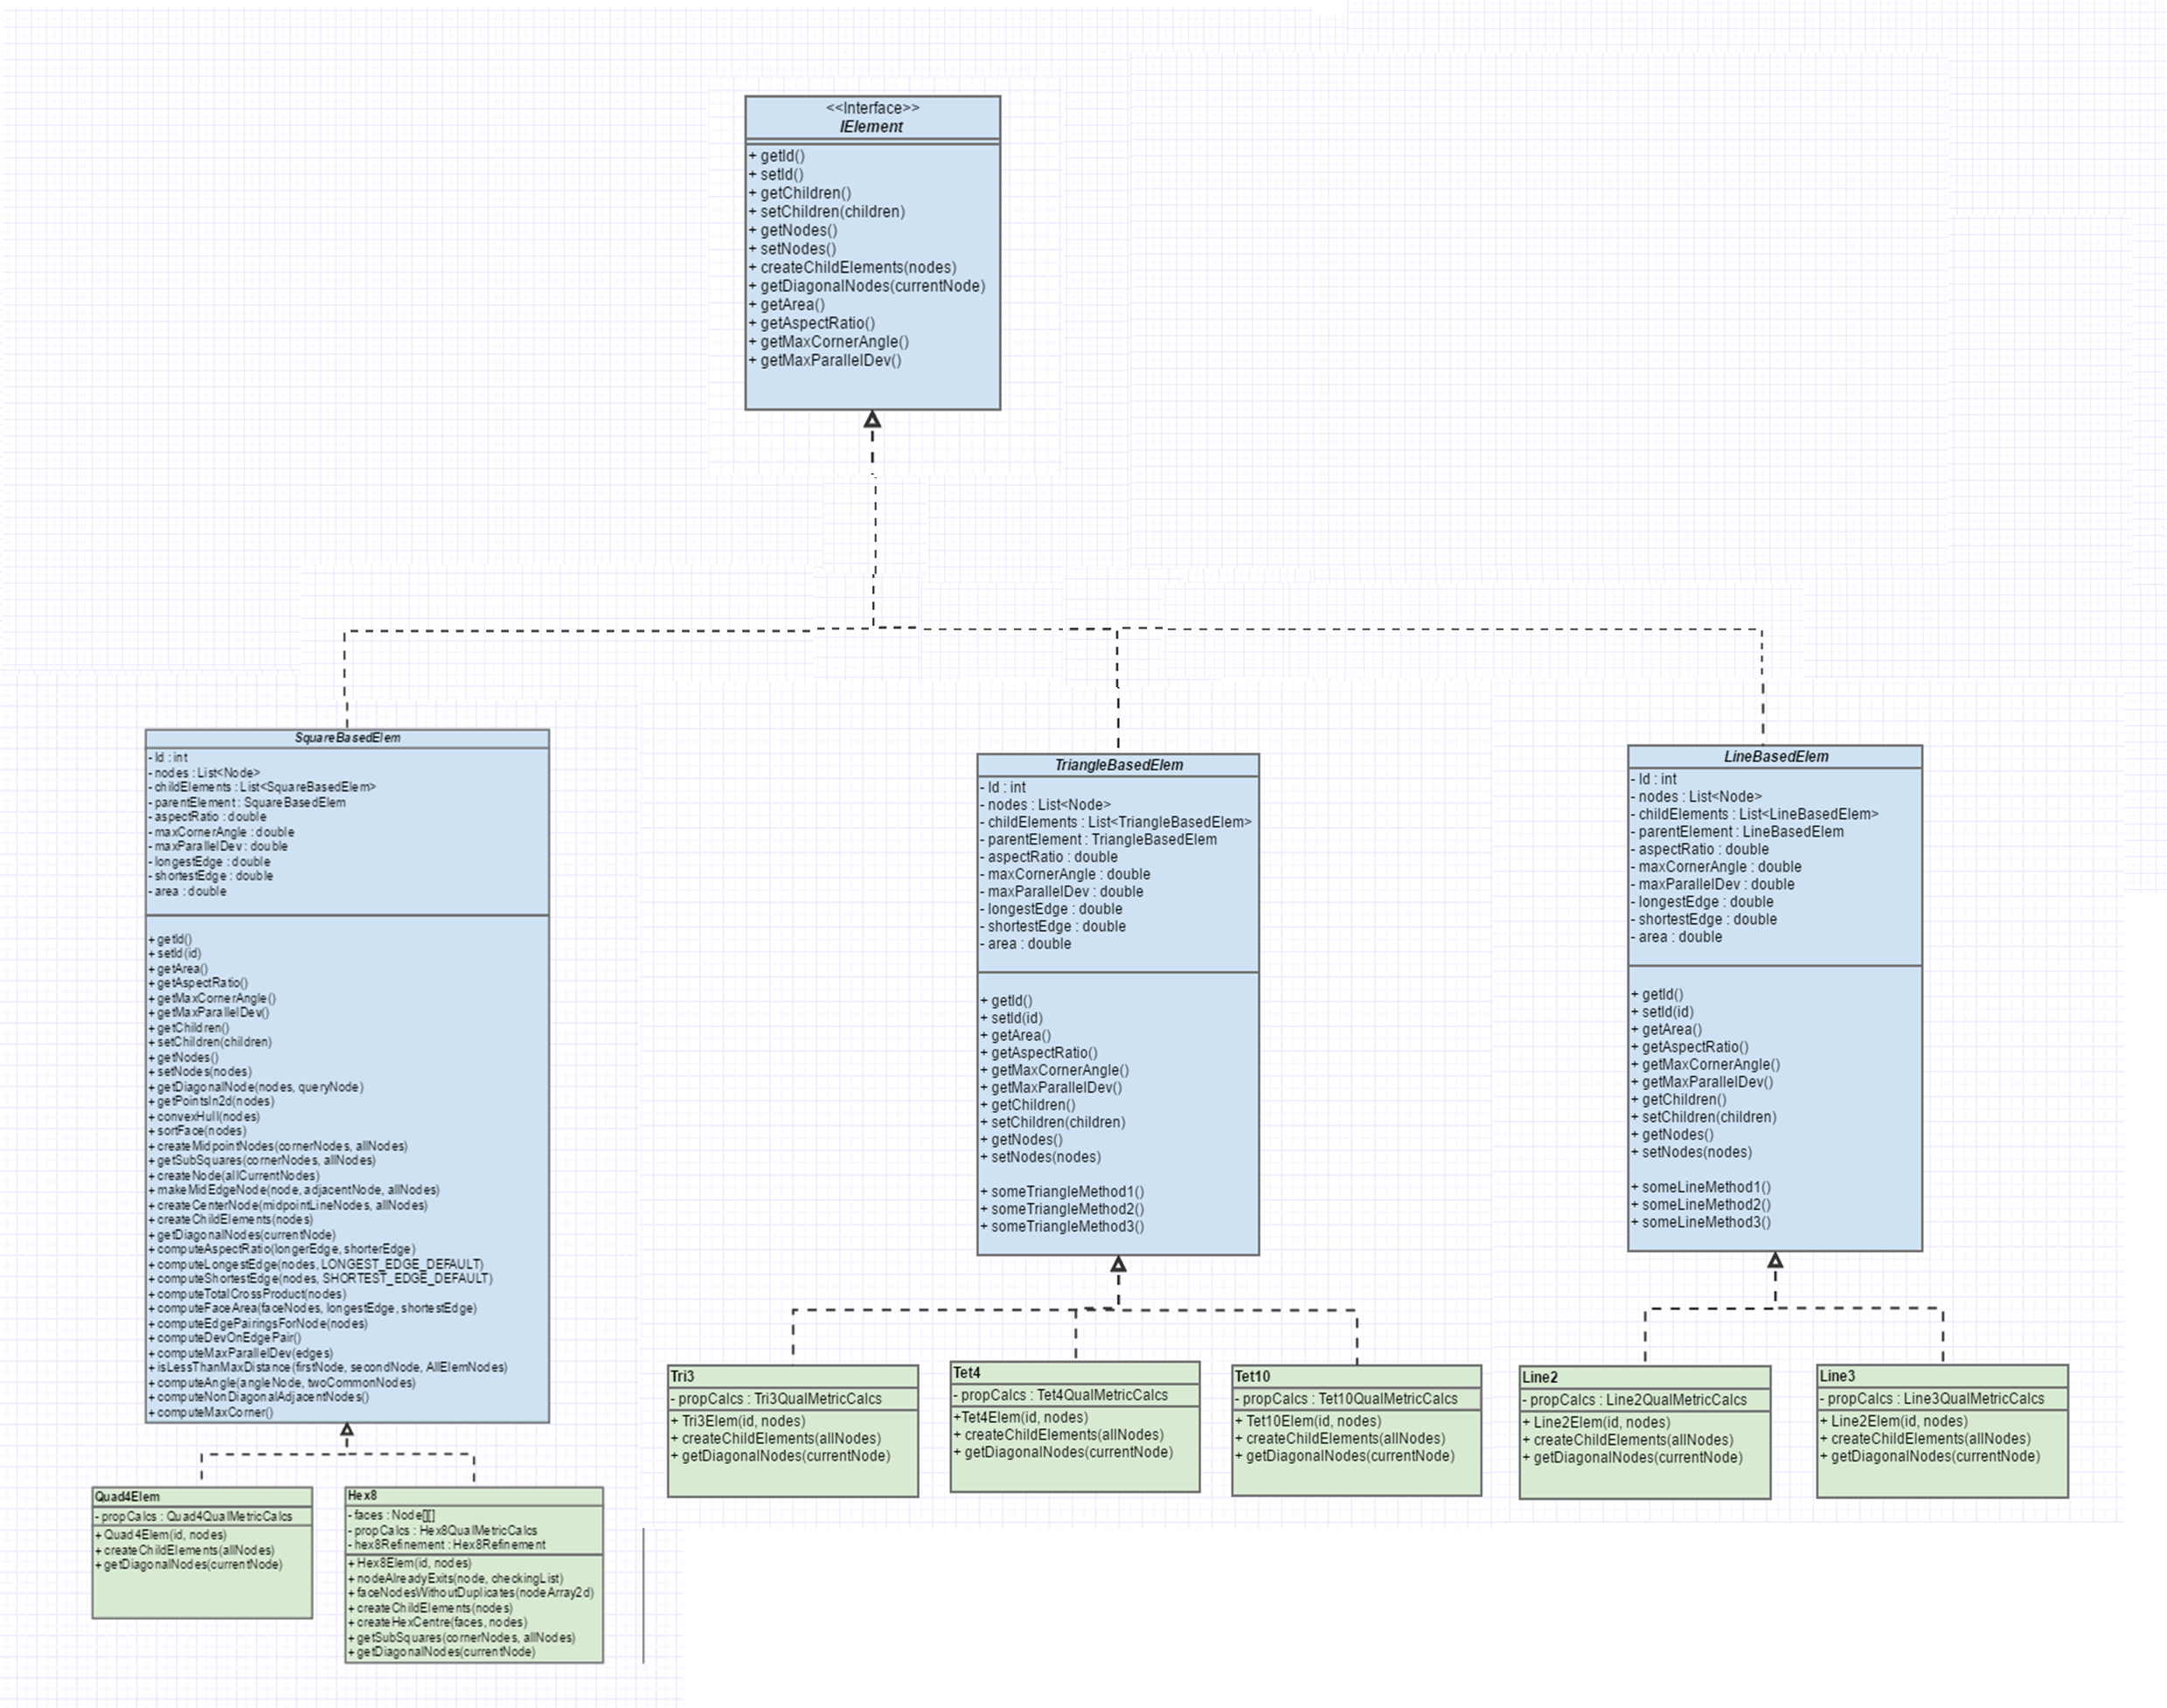
\includegraphics[width=150mm, scale=1]{ElementHigerarchyDiagram2.png}}
  \caption{Class diagram showing the hierarchy of element classification within the data model, due to time limitations I was not able to implement the respective classes for trangle and line based elements, to see image representations of each element type within this class diagram refer to element type appendix}
  \label{fig:h-refinementImp}
\end{figure}


\section{Software Implementation}
The following subsections detail the implementation of the final software solution that has been written to meet the objectives posed at the beginning of this dissertation.

\subsection{Third Party FE Application}
In order to demonstrate the potential feasibility of the hybrid approach it was first important to obtain a finite element solver which could be given a FE model containing data about forces, materials and the mesh structure and then execute the model pro grammatically so as to obtain stress results. \\ 

\noindent
A multitude of commercial FE tools exist with there being a wide variety in both the complexity and cost associated with each tool. 
Finite element software is typically very expensive due to its high development cost and small customer base. Tools used within industry such as ANSYS typically require a great deal of time in order to become proficient in their usage and can cost in excess of five thousand pounds a year for a single licence \cite{AnsysCost}. It was therefore important to find a tool which was both affordable while also powerful enough to demonstrate a working prototype of the re meshing method.
 
\subsection{LISA}
After reviewing several FE applications used within industry in addition to a variety of less well known ones used within academia and by hobbyists LISA  was selected as the solver application for which to implement  the systems prototypes. \\ 

\noindent
\textbf{Strengths: }LISA as a FE tool which allows the user to run models of up to 1300 element for free; This was beneficial in allowing me to experiment with the software and gauge the feasibility of my projects concept before requiring a full version. Once at a stage in the project where each problem had been solved for small models containing less than 1300 elements an academic licence for the software was purchased for the projects use.

LISA also provides a GUI which allows visual inspection of the model and its mesh; This is particularly useful for observing the output of the meshing algorithms which can often provide a human with a much better understanding of how the method has performed and whether or not there are obvious bugs. in the implementation of the meshing procedures \\ 

\noindent
\textbf{Weaknesses: } Due to LISA’s simplicity it does not come with an extensive API allowing for easy programmatic use of its inbuilt features, however it is still possible to interface with LISA through less direct means \cite{LISAManual}. LISA models are stored in .liml files which use XML as a meta mark-up format. The model files contain all the information about the model including the materials used as well as loads and constraints and of course the mesh. It is therefore possible to manipulate a .liml file having parsed its contents before writing a new version of the file which LISA can be called to solve. In order to more easily alter the model it made sense to write a wrapper  for the .liml files to abstract the manipulation of their content.

\subsection{Languages and platforms}
The final system has been written entirely using the C\# programming language (version 5.0) with Visual Studio 2015 as the development environment on a Windows 10 system. C\# is an application development language built on the .NET framework. Although any number of programming languages could have been used to implement the solution C\# offered a good compromise for developing a system with both structural rigidity through static typing and object orientation in addition to functionality to allow for rapid prototyping. C\# does this well through use of LINQ, a part of the standard library that provides a large number of higher order functions which allow for operations to be performed over any data structure that implements the built in IEnumerable interface. Given that much of the code within the project performs the same operation on collections of nodes and elements stored in Lists arrays and dictionaries which all implement IEnumerable the ability to write much of the project using this capability dramatically reduced the number of errors encountered and increased development speed.


\subsection{Implementation Methodology}
Due to the size of the software, which is now in excess of 14000 lines of code it was important to work systematically in order to continuously drive the project in the right direction and avoid the introduction of unnecessary complexity. Through regular reviewal and re factoring this was achieved which dramatically helped to reduced the amount of bugs introduced. \\

\noindent
For the duration of the project the spiral methodology was adhered to. This enforced multiple deliverable stages that were concluded with a supervisor meeting every one or two weeks. Adopting the spiral methodology also provided flexibility regarding the order in which tasks were able to take place outside of a spiral iteration. This was necessary when conducing a research driven project where direction of work for subsequent development iterations was largely driven by the  findings of the work in the previous ones. \\


\noindent
Tasks were chosen every week for the project, the number of tasks and their complexity was determined using a combination of factors including their complexity, the criticality of the task e.g. Did it need to be completed for other important tasks to be started and the time available to me as the individual undertaking the project (More tasks typically performed on weeks when less work was due for other modules.

\subsection{Implementation of Subsystems}
This section describes the implementation details of the various different subsystems which combine to form the overall solution.

\subsubsection{Re-meshing using hierarchical refinement}
Elements within traditional FEA can typically be classified as either triangle or square based elements, each of these provide different strengths and weaknesses when required to mesh and solve models. Within industry triangular elements are typically preferable since it is always possible to generate an initial triangular mesh from any arbitrary CAD geometry algorithmically. This is done by simply making smaller triangles until all gaps along the edge of the geometry are filled \cite{}. The same cannot always be said  when meshing using square elements. For proof of the solutions concept however it was concluded that square based elements were preferable to triangular ones with since the steps required for a basic refinement are much simpler. In addition to this Its also significantly easier to define edges which the ILP rules can be applied to when edges naturally form within a structure through a chain of nodes along the edges of square elements.

%The process of re meshing square based elements 

After reviewing both h-refinement \cite{HandPRefinements} and r-refinement \cite{RRefinement} it was concluded h-refinement would be best the best approach to adopt for use in a due to its simplicity and more widespread use \cite{HandPRefinements} despite the fact that the mesh is usually more computationally expensive than it would have been if it was created using r-refinement \cite{RRefinement}\\ 

Unfortunately Triangular meshes also generally incur a higher computational cost than an equivalent square element mesh due to added complexity of performing the calculations required to remesh in addition to requiring more elements over a given area to achieve the same accuracy.

From an implementation standpoint writing a square based remeshing algorithm is also substantially easier as given an initial mesh made just of square elements the only task is to repeatedly divide each element into four sub elements, by contrast methods uses to re mesh triangular meshes vary greatly are typically more complex and have corresponding initial meshes that are harder to generate manually by human operators \cite{HandMeshing}.

\subsection{Fast node lookup and update of nodes}
A key requirement for the design of the data model generated by the hierarchical re meshing process was the need to perform fast lookup of nodes already present in the mesh. Lookup is important within the meshing methods as a means of checking whether a node that is about to be created already exists within the model, in the event that no such node already exists a new one can be created however if it does then instead of creating a new node the node that already exists needs to be connected to a node in an adjacent element that is currently being refined. \\

\noindent
This issue arose as a result of subdivision for every individual element being a responsibility of that element. From a software engineering perspective was very good since it meant the low level meshing process for each different type of element could be written within that elements class thus avoiding the need for much heavier generalised refinement classes. Most likely these generalised classes would would need to know how to perform the meshing for all elements in the model at once and for each of the different potential element types passed to it as a parameter which is pretty messy. \\ 

\noindent
Consequently despite each Element being capable of meshing itself perfectly when refined elements adjacent to that element also requiring refinement needed the ability to reconnect the new nodes along their edges to those already created by the adjacent element. \colorbox{yellow}{This can be seen below in figure x} \\ 


\begin{figure}
  \centerline{\includegraphics[width=100mm , scale=1]{nodeLinking.png}}
  \caption{The need for an element to check for existing adjacent nodes when subdividing itself during refinement,\\
  	Orange Nodes - An original node for one or more elements \\
	Red Nodes - new nodes made by Elem A \\
	Purple Nodes - new nodes made by Elem B \\
  }
  \label{fig:h-refinementImp}
\end{figure}


\noindent
The solution to this problem was to store all the nodes in the mesh model within a C\# dictionary structure a reference to which is passed to each element within the model. The dictionary can be indexed using a Tuple of the x, y and z coordinates for the new potential element which will either return a node already at that location or indicate that no such node exists, in which case that element is then responsible for creating the node as its first instance. Dictionaries in C\# represent a generalised instance of a hash table ensuring that lookup and insert are both constant time on average.


\subsubsection{hierarchical refinement meshing issue}
A significant issue encountered when working with LISA on the project was an interface requirement specified by LISA requiring nodes for each type of element to be sorted in a specific geometric order. The general rule for node ordering within LISA is to order the nodes as a perimeter around an element in 3d space without paths between nodes crossing one another internal to the element. When first addressing this problem for simple models using elements of Quad4 type the obvious approach was to think of a simple quadrilateral resembling a square, write an algorithm to handle that as a base case before considering a more complex case. The resulting approach was the following approach:

%do pseudo code for initial approach here
\noindent
This approach was sufficient for the vast majority of elements within the different models, however as model complexity increased multiple iterations of the heuristics resulted in increasingly distorted element shapes, resulting in rejection of elements with incorrectly sorted nodes by LISA. \\
 
\noindent
In order to resolve this issue I needed to research and apply a convex hull algorithm to this problem. The subsequent solution was the following: \\ 

%algo 1

\noindent
Despite the existence of algorithms for generating a convex hull in three dimensions due to the small number of points it made sense to assess the effectiveness of a 2d method first before committing and assess the effectiveness of that for resolving my problem. In order to do this I simply took my Quad4 elements and flattened them to a 2d representation by calculating the maximum delta between the greatest and smallest value on each axis and eliminating the axis with the smallest delta. This proved successful, when applied to the model this successfully removed incorrect ordering from elements that had been particularly skewed. \\ 
	
%algo 2

\noindent
This method has O(n log n) time complexity however due to the size of n being 4 in all cases the complexity of sorting an individual element is constant, with the overall complexity of sorting all elements in the model being O(n) where n is the number of elements.


\subsubsection{Stress Based Refinement}
To focus meshing in areas of high stress each iteration needed to parse the results file from the previous iterations execution of LISA. LISA result files are in csv format by default and contain the displacements and stresses associated with each node within the model once it has been solved.

Once the data in the output file has been parsed meshing can be conducted for high stress areas by averaging the stresses across the whole model and then cross referencing the node Ids in the results which have stresses above the average against the main data model allows a list of elements that can be instructed to refine themselves.


\subsubsection{Rule Based Refinement}
Having successfully implemented an simple stress refinement method the next key step of the systems development was to write a framework for executing each of the ILP rules published by Dolsak in his papers \cite{DolsakPaper91, DolsakPaper94, appOfILPToFEMeshDesign} \cite{ConsultRuleIntelltSystemFE}.

Each rule is represented by a function within the final solution, this closely resembles their represented by Dolsak in his papers. Each of the rules resides within the ``RuleManager" class and takes a number of the defined edges as parameters. Each rule then checks the properties of a particular edge against properties which have been identified through the ILP learning mechanism as being important when the model executes. In cases where the rule takes more than one edge as an argument comparison for the properties of each edge are performed. Where a rule detects a relationship in the model the edge is assigned a value corresponding to its criticality, the value is then used by the meshing procedure to determine how many times it should repeatedly re mesh the elements along that edge.


 the significance of elements along a particular type of edge in determining the accuracy of the model. Some rules look for highly critical relationships  which if found have a high importance assigned to them, 

indicate that additional meshing needs to occur for all elements that border the edge. The amount of meshing that occurs for each of the elements along those edges is specified within each of the rules.

The properties that can exist between two edges when compared are the following:

\begin{itemize}
\item Edges opposite one another - the edges run alongside one another closely
\item Edges posses the same form - 
%finish this

\item Edges are considered the same - to meet this requirement both edges must be almost the same length, opposite one another and posses the same form.

\end{itemize}





\subsubsection{Mesh Quality Assessment}
Dittmers rules for computing the quality of both individual elements and the entire mesh are built into their own ``MeshQualtyAssessments" and ``ElementQualityMetrics" classes, the latter of which is encapsulated within an element object, like with refinement this allows each element to assess its own quality removing the need for additional utility classes containing static methods. \\

%not sure about the last sentence here
Since each element is initialised with the nodes that comprise it, it is also possible to derive all the geometric characteristics and thus its quality metrics upon its initialisation. This allows the metrics for each node to also be calculated upon its initialisation removing the risk of elements returning null when asked for them.


\subsection{Implementation Issues}
Implementation of the design was not without its difficulties, many of which arising as a consequence of unforeseeable complications when implementing the well understood theoretical aspects.


\subsubsection{Sorting Element Nodes in 3d space using convex hull Algorithm}


\subsubsection{Attempts to Automatically Define edges within models}
As discussed under evaluation a core issue faced when conducting analysis of the system was identifying where the system behaves poorly through weakness in the methods or poor design and implementation as opposed to poor output generated as a consequence of poor input by the operator. In order to avoid this issue it was desirable to try and remove user intervention besides the configuration of the initial model. The obvious way by which to do this was automatic identification of interesting edges within the model. A crucial property which made this approach appear promising is the fact that it is known that edge importance directly correlates with the size of the edge and how much force is applied near it, since both this information exists within the data model it should be possible to identify edges from it and generate them automatically for Dolsaks rules to process.


\noindent
In practice there are multiple complications surrounding this, several of these arise from ambiguity in Dolsaks paper regarding what constitutes a an edge which is for example "long" or "important". As a result edges are only able to be defined to the extent that a user has confidence in their understanding of these concepts.


Having considered a method using these properties of the mesh several days were then spent attempting to implement it.

Having done so 

% Say something about storage in dictionary


\section{Evaluation of Project}
Evaluation has been essential in order to conclude the effectiveness of both the algorithms used to solve the problem and the capability of their implementation within the final software solution. In order to do this evaluation has been conducted at several levels ranging from functional requirements for the software specification at the lowest to high level analysis of the programs output which in many cases is hard to define and varies from model to model.

\subsection{testing}
In order to validate the system against many of the functional requirements the system only needs to be run on several basic models with different input configurations, observation of the output demonstrates the systems ability to evaluate the quality of meshes using a range of metrics and refinement occurring as a result of both the stresses induced by the user and on their categorisation of edges. 

\subsection{Non functional testing}



\subsection{Evaluation of the system running for various models}
Although the main implementation for this project was the system capable of performing the tasks described above on very simple structures such as a cantilever beam, to demonstrate general applicability with regards to real engineering problems demanded the creation of several models resembling basic equivalents of structures that FE methods would be used on within real engineering analysis. In order to do this and validate the heuristic component against the results obtained in academic papers two of the three models were based on those previously used by Dolsak (Paper mill and Cylinder structures) The third suspension bridge model which was developed specifically to demonstrate its potential capabilities beyond that of the simplistic verification structures.

These initial models were constructed manually using LISA's graphical user interface given some basic measurements by Dolsak and in the case of the suspension bridge from documents available on the web \cite{Dolsak91} \cite{SuspensionBridgeMeasurements}.

\subsubsection{Suspension Bridge structure}


\noindent
The basic bridge structure consists of 196 elements and 212 nodes, which is very coarse for a FE mesh structure. \\


\noindent
The primary model for which work on the latter half of the project was based upon was the following suspension bridge model:


\begin{figure}
  \centerline{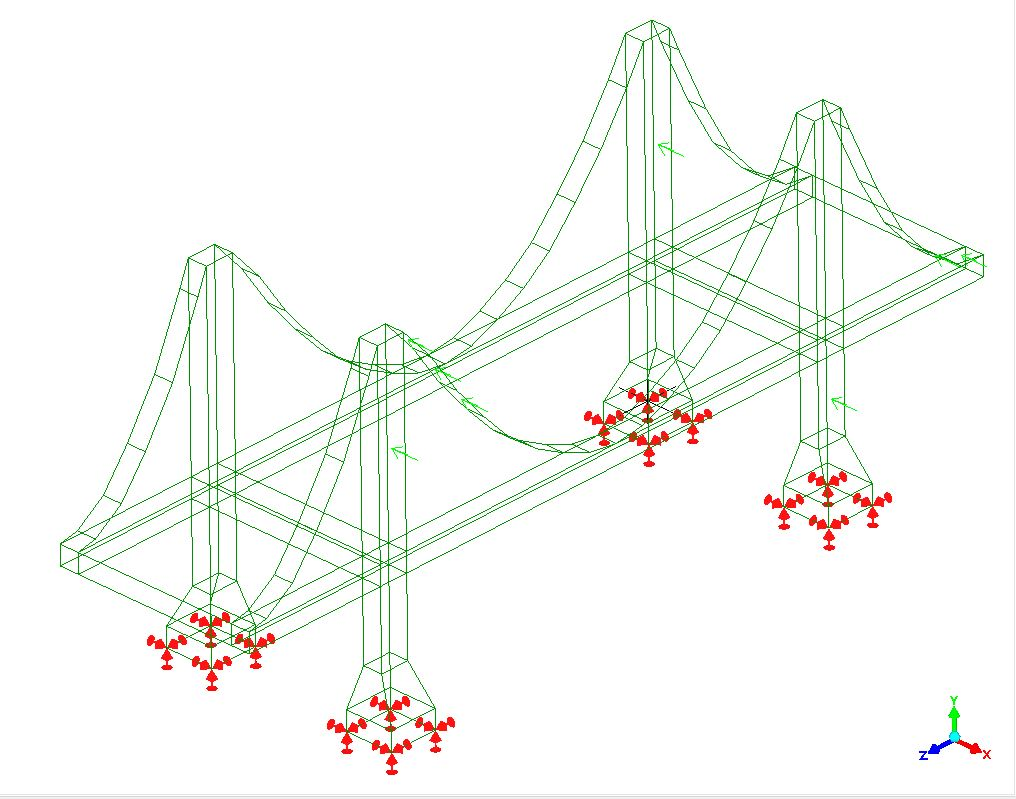
\includegraphics[width=150mm, scale=1]{BasicBridge.jpeg}}
  \caption{Diagram representing the general structure of the system with interactions between non internal entities such as files and LIA shown using dashed lines}
  \label{fig:h-refinementImp}
\end{figure}


\newpage


\noindent
One of the bridge models strengths was it provided high versatility when testing the software solution for m since simulation could be run with forces placed on a range of different faces with corresponding edge rules and a range of varying results obtained. For example a force on the desk of the bridge could be used to simulate the weight of a vehicle moving over it while forces placed sideways on the towers and cables could be used to model stress induced from strong crosswinds.

\subsubsection{Evaluation of bridge for crosswinds}
Simulating crosswinds provided an opportunity  to test the system when simulating a scenario that could feasibly effect the structure.

%typical significance of crosswinds on suspension bridges
%some general forces and on which part of the bridge are they exerted,
%Image showing the forces placed on the actual bridge and possibly on a diagram from some engineering company.
%Where is stress expected to be induced.
\cite{CrosswindsOnSuspensionBridges}

In order to mesh successfully in order to focus refinement on these areas the following rules can be suggested for the bridge structure when crosswinds are applied from a negative x direction.



\subsubsection{Evaluation of bridge for base loading}
Loading the base of a bridge is yet another typical analysis conducted within civil engineering. The loading can be used to represent anything which moves over the bridge that needs to be supported by it such as vehicles or pedestrians. 
\colorbox{yellow}{Given the size of out bridge as x we  can apply a force representing that of a typical number of vehicles moving over the bridge.} 



\colorbox{yellow}{both of these scenarios when used to evaluate the effectiveness of the implementation}

\subsubsection{Validating system against previously obtained research results}
Due to a lack of specific implementation details provided by Dolsak and Muggleton in their papers for generating meshes it was important to demonstrate that the underlying implementation for generating meshes based upon the rules was essentially equivalent. \\ 


Dolsak did however provide information about the various models 

this the models used by Dolsak in order to train his initial ILP system responsible for generating the rules were re crated. This allowed for verification of the heuristic component of the project through comparison of both implentations outputs. \cite{DolsakPaper91}.


\subsubsection{Paper Mill}

\begin{figure}
\centering
\begin{subfigure}{.5\textwidth}
  \centering
  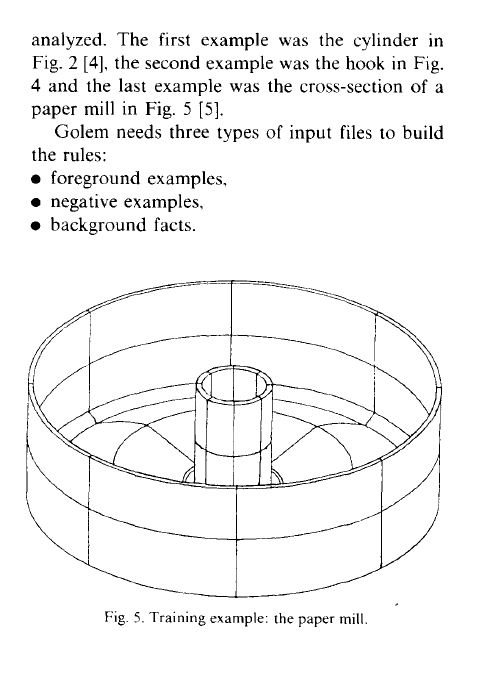
\includegraphics[width=0.9\linewidth]{PaperMillDolsak.jpeg}
  \caption{Paper Mill presented by Dolsak in his paper as input for training Golem}
  \label{fig:sub1}
\end{subfigure}%
\begin{subfigure}{.5\textwidth}
  \centering
  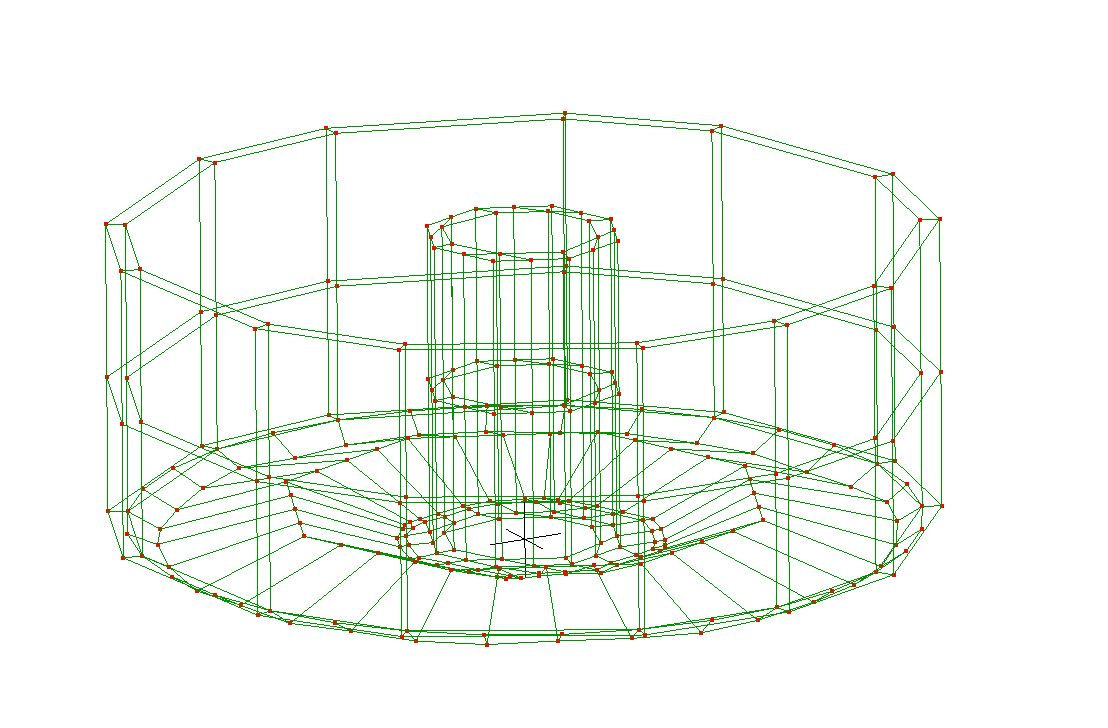
\includegraphics[width=0.9\linewidth]{PaperMillWithinLisa.jpeg}
  \caption{Representation of paper mill within LISA before applying meshing rules to validate}
  \label{fig:sub2}
\end{subfigure}
\label{fig:test}
\end{figure}


\subsubsection{Cylinder}
Obtaining results based on the edge relationships described within the research literature was the first step required when performing evaluation of the cylinder. The rules provided in Dolasks paper used to generate the initial JSON file were the following:




\begin{figure}
\centering
\begin{subfigure}{.5\textwidth}
  \centering
  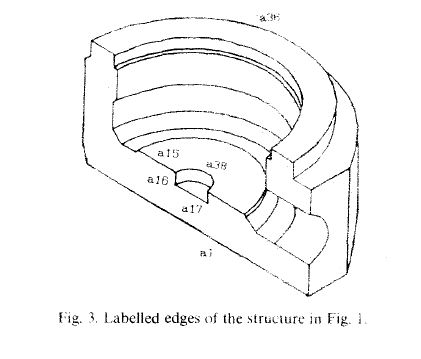
\includegraphics[width=0.9\linewidth]{DolsakCylinderWithEdges.jpeg}
  \caption{Cylinder model used by Dolsak with edges labeled, each labelling corresponds to a rule generated by the Golem algorithm \cite{DolsakPaper91}}
  \label{fig:sub1}
\end{subfigure}%
\begin{subfigure}{.5\textwidth}
  \centering
  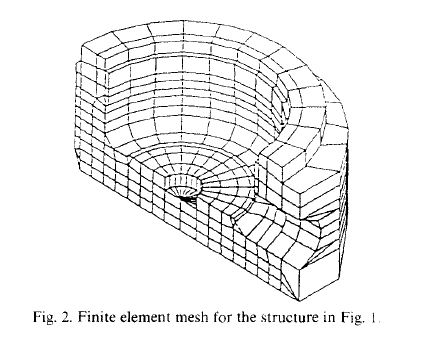
\includegraphics[width=0.9\linewidth]{DolsakCylinderMeshed.jpeg}
  \caption{Diagram representing the general structure of the system with interactions between non internal entities such as files and LIA shown using dashed lines}
  \label{fig:sub2}
\end{subfigure}
\label{fig:test}
\end{figure}

The resulting mesh generated by the system after increasing numbers of iterations based primarily

\begin{figure}
\centering
\begin{subfigure}{.5\textwidth}
  \centering
  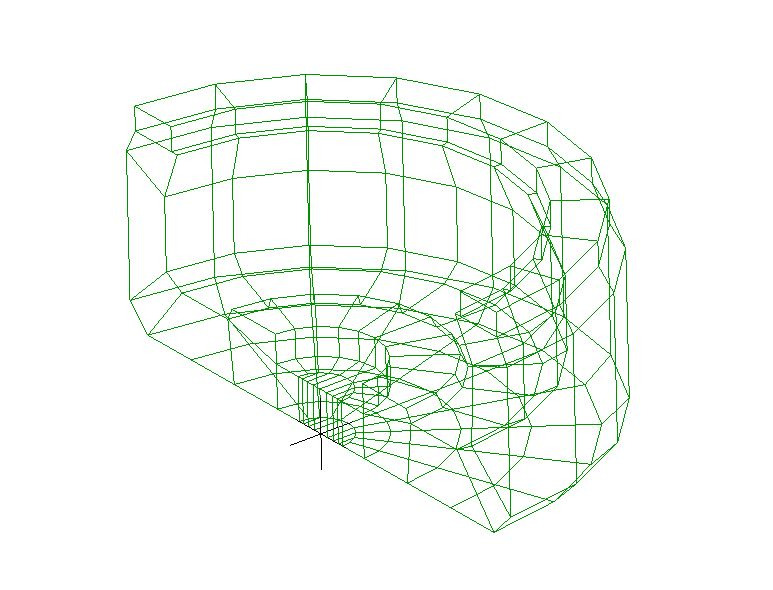
\includegraphics[width=0.9\linewidth]{DolsakCylinderWithinLisa.jpeg}
  \caption{Cylinder cross section initial construction within Lisa \cite{DolsakPaper91}}
  \label{fig:sub1}
\end{subfigure}%
\begin{subfigure}{.5\textwidth}
  \centering
  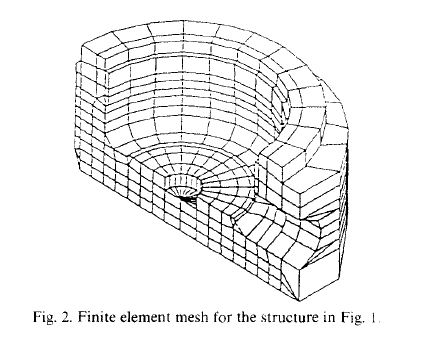
\includegraphics[width=0.9\linewidth]{DolsakCylinderMeshed.jpeg}
  \caption{Diagram representing the general structure of the system with interactions between non internal entities such as files and LIA shown using dashed lines}
  \label{fig:sub2}
\end{subfigure}
\label{fig:test}
\end{figure}




\newpage

\section{Evaluation of testing on models}
Executing the three main models with a range of simulation conditions formed the bulk of my system level testing for the project.




\subsection{Evaluation of Subsystems based on model evaluation}
Having run the system on the range of models described above it was possible to begin assessing it's ability to mesh and the use of Dittmers metrics for assessing 
the quality of each mesh.

\subsubsection{Analysis of Dittmer mesh quality metrics}
When evaluating Dittmers metrics for distinguishing between meshes of different qualities there were several key observations about the metrics in particular which resulted in re assessment of how to evaluate the mesh qualities in general.
Central to these observations was that although metrics provided by Dittmer give a clear indication of the general accuracy of stress across a mesh or a particular element in the majority of cases they give no further insight into the strengths of the particular element arrangement within a given mesh. Consequently it was possible to demonstrate that the meshes produced as a result of the methods retailed general quality that is desired within general meshes but not that the mesh was especially good given the particular model it was based on. \\


\noindent
After evaluating these initial results it became clear that demonstrating the quality of mesh tailoring would be a harder task than originally conceived requiring. It became clear that a metric for demonstrating this property would involve calculating the similarity of the resulting mesh to some hypothetical ideal for the model.

Additional research revealed that generally this conclusion was generally agreed upon by both academics and industrial users of mesh quality metrics. With the difficulty lying in the design of metrics which are consistent indicators of quality across a wide range of geometries they are typically used as a means of validating a is not of poor quality although not necessarily of high.

As the first known system that performs this type of hybrid remeshing it therefore made sense to attempt development of a metric which although could not be used to compare the quality of resulting meshes to those produces by different tools would be useful for contrasting the quality of the meshes that were produced by the system.


%Subsequent research suggested




\subsubsection{Evaluation of stress based remeshing}



\subsection{Increase in performance through parallel execution}
The following 

The average speed up (Time of serial execution/ Time of parallel execution) was 


The Efficiency of the parallel execution (speedup / number of processors) with an Intel i5 processor with 4 cores the average efficiency  was calculated as

\subsection{Quality}
The quality of the design and implementation of the system reflects my ability not only as a computer science undergraduate but as a developer with one year industrial experience, although not directly effecting the execution of the program properties such as appropriate variable naming, loose coupling of classes, use of abstractions and descriptive error messages make the software easier to read and debug for any potential future developers.


\subsection{Documentation}
The process of continuously writing descriptive documentation was important to the success of the project and was treated as an integral part to meeting to the goals of the project development methodology which aimed to reduce the systems complexity and improve readability. Through the writing Doc comments corresponding to every function within the codebase it was possible to generate documentation files automatically through use of the tool Doxygen. This allows anyone with the solution to view descriptions of each of its functions either in the codebase or alternatively through the manual produced automatically by Doxygen.

\subsection{Maintainability}
As a result of loosely coupled design with each file containing only one class and each class and function written with the goal of providing only one item of functionality. the 

and well written documentation the system is for the most part maintainable. 


\subsubsection{Evaluation Issues}
A significant issue faced in attempting to demonstrate the effectiveness of the system was to provide an indication of how well the system worked without taking into account the ability of the user who may be providing the edge rules for a particular model. Not taking this into account would result in an inaccurate representation of its ability.

\subsection{Evaluation of overall project}

% Overall the project met all its initial requirements laid out in both the objectives and its requirements.
% 


\subsection{Evaluation summary}

\subsection{Successes and Limitations}


\section{Further Work}
This section details some areas which given additional time to work on the project would at the very least be investigated, if not implemented. Each of these areas would hopefully provide some benefit in assisting to demonstrate the possibilities of hybrid methods.

\subsection{Gathering feedback from experienced engineers}
Approaching the end of the project it became clear that in order to better identify the systems strengths and weaknesses would require additional user testing by engineers who have experience conducting this type of analysis. Despite not having the available time to conduct user feedback I maintained contact throughout the project with a variety of acquaintances I was able to make through my industrial placement year at gas turbine manufacturer Rolls-Royce, with several expressing interest in the concept. Combining feedback from engineers with extensive applied industrial experience and that of academics within the universities own mechanical engineering department would hopefully have allowed for a more conclusive analysis of the systems overall capabilities. Obtaining user feedback was not considered feasible given the amount of time to implement the project and the already inherent complexities in producing a working implementation for just a few test cases. As such even if time had been available the ethical clearance required to collect user feedback at the start was not obtained.


\subsection{Improving usability through a web interface}
Although possible to visit various engineers in order to conduct feedback the process is both time consuming on my part and inconvenient for the participant as a rigid time for which to meet must be scheduled and a laptop containing the working software brought to them which they must design or transfer their model to before running it multiple times to obtain results. This scenario is at best inconvenient for the participants and pressures them into arriving at a conclusion within a relatively small time of experimenting with it. \\ 

\noindent
Instead by facilitating interaction with the system by means of a web interface the engineers would be able spend as little or as much time as they like experimenting with the system and allow them to submit feedback digitally. This would potentially allow feedback to be obtained from  a much wider range of different sources separated by significant geographic distance. \\\ 

\noindent
In order to theoretically use such an interface each engineer would simply have to download the free version of LISA from the following webpage \url{http://www.lisafea.com/index.html} import a model they already have which is less than 1300 elements(LISA supports imports from multiple CAD formats including Standard for the Exchange of Product model data (STEP) and Initial Graphics Exchange Specification (IGES)) \cite{LISAReference} and then submit this along with a JSON file containing edges they have designated as important for their model. Upon receiving the request the web server would the current project with their input data and having finished allow them to download the re meshed model along with the calculated stress data for analysis.


\section{Personal Reflections and Summary}

Comparing the current progress of the project against the plan things are on track to be completed as scheduled. So far I am pleased with both my research efforts and the functionality that I have been able to implement. My primary concern at present is that the ILP generated rules may not perform as well as expected when fully implemented or that they perform well but only for a limited set of geometries, which would be disappointing. While conducting research, development and implementation for the project I have worked methodically to best understand each problem as and when they occur and consider each of the possible solutions before committing to one. I feel this approached has saved me much time and has forced me to reach a better view about what exactly each subsystem should do and how to implement it. In hindsight if I were to repeat the first part of the project again I would have organised my time differently to spend less of it focussed on the details of coursework assignments for other modules into making further progress on the implementation of the rule system.

\newpage
\pagestyle{empty}
\begin{landscape}
\vspace*{1cm}
\hspace*{-3cm}
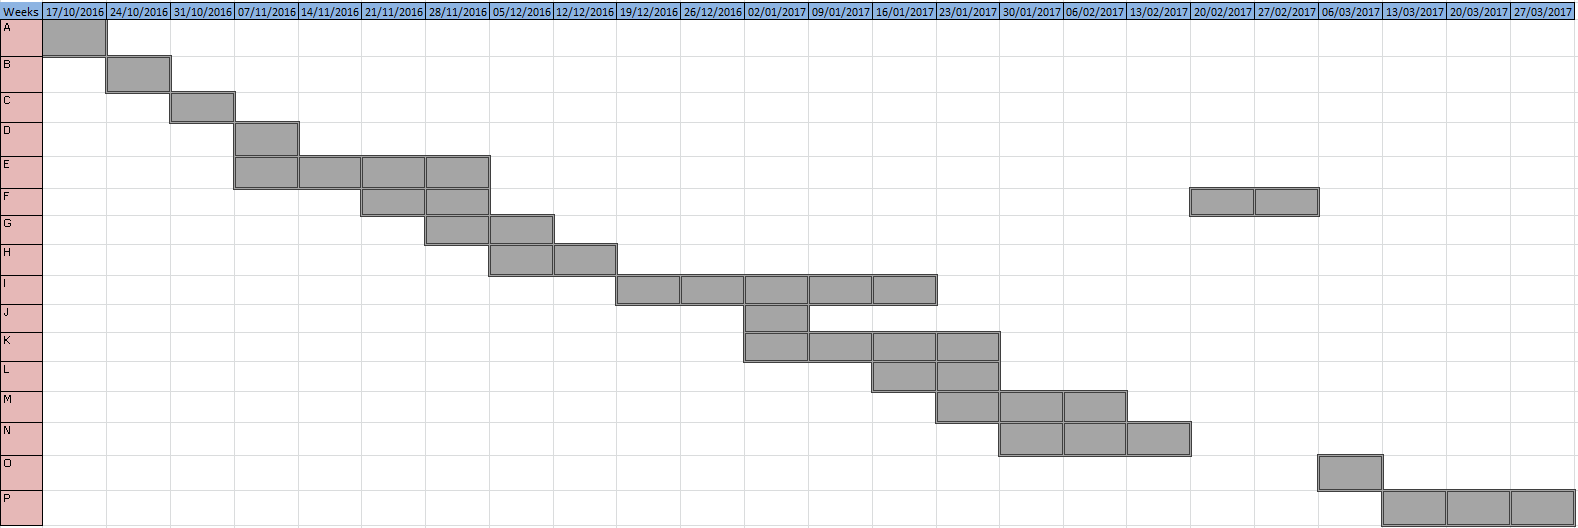
\includegraphics[width =700px, height=300px]{TimePlanUpdated2.png} \par
\hspace*{-1cm}

\end{landscape}

\newpage

\begin{changemargin}{\CMwidth}{\CMheight} 

\addcontentsline{toc}{section}{References}
\begin{thebibliography}{9}

\bibitem{cite0} Max D. Gunzburger, Janet S. Peterson \emph{Finite Element Methods} \url{https://people.sc.fsu.edu/~jburkardt/classes/fem\_2011/chapter1.pdf}

\bibitem{HandPRefinements} Adaptive Finite Element Techniques \url{http://www.cs.rpi.edu/~flaherje/pdf/fea8.pdf}

\bibitem{RRefinement} Scott McRae \emph{r-Refinement grid adaptation algorithms and issues}

\bibitem{DolsakPaper91} Bojan Dolsak and Anton Jezernik \emph{Mesh generation expert system for engineering analysis with FEM}

\bibitem{DolsakPaper94} Bojan Dolsak, Anton Jezernik \emph{A knowledge base for finite element mesh design} Artificial Intelligence in Engineering 9 (1994)

\bibitem{appOfILPToFEMeshDesign} Bojan Dolsak, Stephen Muggleton \emph{The Application of Inductive Logic Programming to Finite Element Mesh Design}

\bibitem{ConsultRuleIntelltSystemFE} Bojan Dolsak, Frank Reig, Reinhard Hackenschmidt \emph{Consultative Rule-Based Intelligent System for Finite Element Type Selection} Research Gate 2016

\bibitem{TraditionalHybridRefinement} Paul Dvorak \emph{Two meshing methods are better than one} \url{http://machinedesign.com/archive/two-meshing-methods-are-better-one}

\bibitem{NeuralNetworks} Larry Manevitz, Malik Yousef, Dan Givoli \emph{Automatic Mesh Generation (for Finite Element Method) Using Self-Organising Neural Networks}

\bibitem{caseBasedReasoning}Abid Ali Khan, Imran Ali Chaudhry2 \& Ali SaroshCase \emph{Case Based Reasoning Support for Adaptive Finite Element Analysis: Mesh Selection for an Integrated System}

\bibitem{MuggletonILP} Stephen Muggleton \emph{Inductive Logic Programming}

\bibitem{Golem} \url{http://www-ai.ijs.si/~ilpnet2/systems/golem.html}

\bibitem{ILPYoutubeLecture}Stephen Muggleton \emph{Logic based and Probabilistic Symbolic Learning} \url{https://www.youtube.com/watch?v=4CwdO5dWW98}

\bibitem{DittmerMeshQualityMet} Jeremy P. Dittmer, C. Greg Jensen, Michael Gottschalk, and Thomas Almy \emph{Mesh Optimisation Using a Genetic Algorithm to Control Mesh Creation Parameters}

\bibitem{PoorFEElementShapes} \url{http://danielpeter.github.io/rays.html}

\bibitem{cite03} Lina Vasiliauskiene, Romualdas BAUŠYS \emph{Intelligent Initial Finite Element Mesh Generation for Solutions of 2D Problems} INFORMATICA, 2002, Vol. 13, No. 2, 239–250 2002

\bibitem{cite04} E.Bellengera,Y.Benhafidb, N.Troussierb \emph{Framework for controlled cost and quality of assumptions in finite element analysis} Finite Elements in Analysis and Design 45 (2009) 25--36

\bibitem{IntroductionToFE} G. P. Nikishkov \emph{INTRODUCTION TO THE FINITE ELEMENT METHOD} \url{http://homepages.cae.wisc.edu/~suresh/ME964Website/M964Notes/Notes/introfem.pdf}

\bibitem{LISAManual} \url{http://www.lisafea.com/pdf/manual.pdf}

\bibitem{cite06}Nam-Ho Kim \emph{STRUCTURAL DESIGN USING FINITE ELEMENTS} http://web.mae.ufl.edu/nkim/eas6939/Opt\_FEM.pdf

\bibitem{cite07}\emph{Type of Finite Elements and Steps in FEA Process}\\
http://highered.mheducation.com/sites/dl/free/0073398144/934758/\\Ch07TypesOfFiniteElementsAndStepsInFEAProcess.pdf 

\bibitem{cantileverBeam} \url{https://www.quora.com/What-is-the-cantilever-beam-What-is-the-advantages-and-disadvantages-of-it}

\bibitem{LISAWebsite} \url{http://www.lisafea.com/purchase.html}

\bibitem{Doxygen} \url{http://www.stack.nl/~dimitri/doxygen/} 

\bibitem{ElementShapeQuality} \url{https://caeai.com/blog/will-poorly-shaped-elements-really-affect-my-solution}

\bibitem{AnsysCost} \url{http://mscnastrannovice.blogspot.co.uk/2013/04/how-much-does-ansys-cost.html}

\bibitem{HighStressCorner} \url{http://www.engineeringanalysisservices.com/moving-mesh-fea-analysis.php}

\bibitem{CSharpConvexHull} \url{http://loyc.net/2014/2d-convex-hull-in-cs.html}

\end{thebibliography}

\end{changemargin}

\end{document}
